\documentclass{optica-article}

\journal{opticajournal}

\articletype{Research Article}

\usepackage{lineno}
\usepackage{graphicx}
\usepackage{amsmath}
\usepackage{amssymb}
\usepackage{color}
\usepackage{hyperref}
\hypersetup{
    colorlinks=true,
    linkcolor=blue,
    filecolor=magenta,
    urlcolor=cyan,
    pdftitle={Machine Learning-Enhanced Entanglement Characterization},
    pdfauthor={S.K. Rithvik, R.P. Singh, Shashi Prabhakar},
    pdfsubject={Quantum State Characterization},
    pdfkeywords={quantum entanglement, machine learning, quantum state tomography}
}
\usepackage{float}
\linenumbers

\begin{document}

\title{Machine Learning-Enhanced Entanglement Characterization in Bi-partite Ququart Systems}

\author{S.K. Rithvik,\authormark{1,2} R.P. Singh,\authormark{1} and Shashi Prabhakar\authormark{1}}

\address{\authormark{1}Atomic, Molecular and Optical Physics Division, Physical Research Laboratory, Navrangpura, Ahmedabad 380009, India\\
\authormark{2}Indian Institute of Technology Gandhinagar, Palaj, Gandhinagar 382355, India\\
}

\email{\authormark{*}rithvik1122@gmail.com}

\begin{abstract*} 
We present a comprehensive comparative study between machine learning and traditional approaches for characterizing entanglement in bi-partite ququart systems. While conventional quantum state tomography requires $D^2$ measurements for a complete reconstruction, we demonstrate that deep learning techniques can achieve comparable accuracy with significantly fewer measurements. Our research evaluates three neural network architectures—Multi-Layer Perceptron (MLP), Convolutional Neural Network (CNN), and Transformer Network—against classical Maximum Likelihood Estimation (MLE) and Bayesian methods. The neural approaches achieve up to two orders of magnitude faster computation times while maintaining competitive accuracy in estimating entanglement negativity. Notably, with 400 measurements, our Transformer architecture achieves a mean squared error of $7.01 \times 10^{-3}$ in sub-second inference time, compared to $2.95 \times 10^{-3}$ for MLE requiring over 60 seconds. All methods demonstrate $1/\sqrt{N}$ scaling in error reduction with increased measurements, confirming theoretical predictions while highlighting the computational efficiency advantages of neural approaches. This work presents a significant advancement toward real-time entanglement characterization, particularly relevant for higher-dimensional quantum systems where traditional methods become computationally prohibitive.
\end{abstract*}

\section{Introduction}

Quantum entanglement, first termed by Schrödinger\cite{Schrödinger_1935} in response to the Einstein-Podolsky-Rosen (EPR) paradox\cite{PhysRev.47.777}, represents a fundamental departure from classical physics and serves as a critical resource for quantum technologies. The characterization of entanglement in high-dimensional systems, particularly bi-partite ququarts, presents significant experimental and computational challenges\cite{RevModPhys.81.865}. Traditional approaches rely on quantum state tomography, which becomes exponentially expensive with system size\cite{Torlai2018}.

This work addresses a fundamental question: Can we achieve reliable entanglement characterization with fewer measurements using machine learning techniques? Recent advances in deep learning\cite{LeCun2015} and attention mechanisms\cite{Vaswani2017} have shown promising results in quantum state characterization\cite{transformer_quantum_2022,doi:10.1126/sciadv.add7131}. We focus on bi-partite ququart systems, using entanglement negativity as our metric, and compare various computational approaches in terms of both accuracy and efficiency.

The rapid advancement of quantum technologies necessitates efficient methods for characterizing quantum states and their properties. Conventional approaches become increasingly impractical as system dimensionality grows, motivating our investigation of machine learning alternatives that can learn efficient representations of quantum data. Our approach combines techniques from quantum tomography, statistical estimation, and modern deep learning to develop a comprehensive framework for entanglement characterization.

\section{Methods}

\subsection{Quantum Framework and Data Generation}

The entanglement negativity $\mathcal{N}(\rho)$ for a quantum state $\rho$ is defined as:

$$ \mathcal{N}(\rho) = \frac{||\rho^{\Gamma_A}||_1 - 1}{2} $$

where $\rho^{\Gamma_A}$ represents the partial transpose with respect to subsystem A, and $||X||_1 = \text{Tr}\sqrt{X^\dagger X}$ is the trace norm. For bi-partite ququarts, $\mathcal{N}(\rho)$ ranges from 0 for separable states to 1.5 for maximally entangled states.

Our implementation, as shown in the \texttt{entanglement\_negativity} function, carefully handles numerical stability issues by filtering out small imaginary components (threshold $10^{-10}$), ensuring eigenvalues are finite, and gracefully handling potential linear algebra errors with appropriate fallbacks.

Our measurement protocol utilizes five mutually unbiased bases (MUBs) for each subsystem, implemented in the \texttt{generate\_mubs} function:

\begin{itemize}
\item $M_0$: Standard computational basis ($I_4$)
\item $M_1$: Hadamard-like basis with real coefficients, constructed as a balanced superposition with specific phase patterns
\item $M_2, M_3, M_4$: Complex-valued bases with carefully designed phase relationships to ensure mutual unbiasedness
\end{itemize}

The complete set of POVMs is constructed in the \texttt{construct\_povms} function through a systematic approach:
\begin{enumerate}
\item Extracting individual measurement vectors from each basis
\item Forming all possible tensor products between vectors from different subsystems
\item Computing outer products to create valid POVM operators
\item Ranking POVMs by their information content using eigenvalue spread
\end{enumerate}

To ensure robust sampling across the entanglement spectrum, our \texttt{generate\_data\_with\_mixture} function employs a sophisticated stratified sampling approach:

\begin{itemize}
\item Five entanglement bins spanning the full range [0.0, 1.5]
\item Bin-specific purity parameters optimized for target entanglement ranges
\item Adaptive parameter selection with timeouts (120s per bin) to ensure balanced datasets
\item Batch processing (10 states per batch) with dynamic parameter updates
\end{itemize}

State generation combines both pure and mixed state techniques:
\begin{itemize}
\item Pure states: Generated using normalized complex Gaussian vectors (\texttt{randompure} function)
\item Mixed states: Created via Haar random unitaries applied to low-rank operators (\texttt{randomHaarState} function) 
\item Controlled mixing with maximally mixed states to achieve target entanglement values
\item Shot noise simulation with 200 shots per measurement using binomial sampling
\end{itemize}

Our implementation features several optimizations for numerical robustness, including eigenvalue filtering, trace normalization safeguards, and exception handling for pathological cases.

\subsection{Neural Network Architectures}

\subsubsection{Multi-Layer Perceptron (MLP)}

Our MLP architecture, implemented in the \texttt{MLP} class, features several innovations specifically designed for quantum measurement processing:

\begin{itemize}
\item \textbf{Adaptive Architecture Scaling}: The network automatically adjusts its complexity based on input dimensionality:
\begin{itemize}
\item Hidden layer size: $h = \max(1024, \min(4096, input\_size * 32))$
\item This allows the network to efficiently process both sparse measurements (10-20) and dense measurements (250-400)
\end{itemize}

\item \textbf{Measurement-Aware Attention}: The network incorporates an explicit attention mechanism:
\begin{itemize}
\item Implemented as a dedicated sub-module:
\begin{verbatim}
self.input_attention = nn.Sequential(
    nn.Linear(input_size, input_size),
    nn.LayerNorm(input_size),
    nn.Sigmoid()
)
\end{verbatim}
\item This learns to assign importance weights to each measurement
\item Weights are applied via element-wise multiplication: $x = x * weights$
\end{itemize}

\item \textbf{Physics-Aware Initialization}: Weight initialization scales with the measurement count:
\begin{itemize}
\item Scale factor: $1.0/\sqrt{input\_size}$
\item Output layer: Small initial weights ($gain=0.01$)
\item Hidden layers: Uniform initialization scaled by $\max(0.05, scale\_factor)$
\item This prevents vanishing/exploding gradients regardless of measurement count
\end{itemize}

\item \textbf{Progressive Feature Refinement}: The main processing pipeline uses:
\begin{itemize}
\item Input batch normalization to standardize measurements
\item GELU activation for smooth gradients
\item Measurement-dependent dropout: $p = \max(0.05, 0.2 - 0.001 * input\_size)$
\item Progressive dimension reduction: $h \rightarrow h/2 \rightarrow h/4 \rightarrow 1$
\end{itemize}
\end{itemize}

This architecture automatically adapts to different measurement counts while maintaining robust training dynamics, making it particularly effective across diverse experimental scenarios.

\subsubsection{Convolutional Neural Network (CNN)}

The CNN architecture, defined in the \texttt{CNN} class, employs spatial projection and multi-scale feature extraction:

\begin{itemize}
\item \textbf{Adaptive Spatial Projection}: Measurements are mapped to a 2D grid:
\begin{itemize}
\item Grid dimension: $grid\_dim = \lceil\sqrt{input\_size}\rceil$
\item Zero-padding ensures consistent dimensionality: \\ $x = F.pad(x, (0, grid\_dim^2 - x.size(1)))$
\item Reshaping: $x.view(batch\_size, 1, grid\_dim, grid\_dim)$
\end{itemize}

\item \textbf{Measurement-Scaled Feature Maps}: Filter counts adapt to measurement complexity:
\begin{itemize}
\item Base filters: $min(128, \max(32, input\_size / 2))$
\item This ensures efficient representation for both small and large measurement counts
\end{itemize}

\item \textbf{Residual Convolution Blocks}: Three specialized blocks:
\begin{itemize}
\item Each block contains two convolutional layers with batch normalization
\item Residual connections: $x = F.relu(x + identity)$
\item Progressive downsampling: Full resolution → Half → Quarter
\item Channel scaling: Base → 2$\times$Base → 4$\times$Base
\end{itemize}

\item \textbf{Multi-Scale Feature Integration}: Features are combined via:
\begin{itemize}
\item Adaptive pooling to 4$\times$4 feature maps
\item Channel-wise concatenation of features from different scales
\item Three-stage regression head with batch normalization and ReLU activation
\end{itemize}
\end{itemize}

The CNN's architecture leverages spatial relationships between measurements through its convolutional structure, enabling it to capture both local and global correlations in the measurement data.

\subsubsection{Transformer Network}

Our Transformer architecture, implemented in the \texttt{Transformer} class, represents the most sophisticated approach, incorporating several advanced techniques:

\begin{itemize}
\item \textbf{Adaptive Embedding}: The embedding dimension scales with measurement count:
\begin{itemize}
\item $embed\_dim = \min(512, \max(128, input\_size * 4))$
\item Attention heads: $n\_heads = \min(8, \max(4, embed\_dim / 64))$
\item This ensures the model capacity matches input complexity
\end{itemize}

\item \textbf{Specialized Measurement Embedding}:
\begin{itemize}
\item Individual measurement projection: $nn.Linear(1, embed\_dim)$
\item Layer normalization for stable gradients
\item Measurement-dependent dropout: $\max(0.05, 0.15 - 0.0005 * input\_size)$
\end{itemize}

\item \textbf{Advanced Positional Encoding}:
\begin{itemize}
\item Implemented as sinusoidal encodings with 5000 position capacity
\item Frequency spans logarithmic range for multi-scale temporal sensitivity
\item Added to embeddings: $x = x + self.pos\_encoding[:, :N, :]$
\end{itemize}

\item \textbf{Explicit Measurement Attention}:
\begin{itemize}
\item Learnable parameter matrix: $self.measurement\_attn = nn.Parameter(...)$
\item Applied via sigmoid activation for stable training
\item Initialized with slight randomness to break symmetry
\end{itemize}

\item \textbf{Measurement-Aware Transformer Blocks}:
\begin{itemize}
\item Layer count scales with measurements: $n\_layers = \min(8, \max(2, input\_size / 32))$
\item Feed-forward dimension: $ff\_dim = embed\_dim * 4$
\item Pre-normalization architecture for training stability
\item GELU activation for smoother gradients
\end{itemize}

\item \textbf{Sophisticated Output Aggregation}:
\begin{itemize}
\item Weighted pooling across measurement dimension
\item Weights computed via softmax with embedding-scaled normalization
\item Three-stage output head with layer normalization and GELU activation
\end{itemize}
\end{itemize}

The Transformer's self-attention mechanism allows it to dynamically focus on the most informative combinations of measurements, making it particularly effective at extracting maximal information from limited measurement data.

\subsection{Classical Estimation Methods}

\subsubsection{Maximum Likelihood Estimation (MLE)}

Our MLE implementation, through the \texttt{\_single\_mle\_estimation} and \texttt{parallel\_mle\_estimator} functions, employs a sophisticated approach to density matrix reconstruction:

\begin{itemize}
\item \textbf{Core Algorithm}: The iterative process follows:
\begin{itemize}
\item Initialization: Maximally mixed state $\rho_0 = I/16$
\item For each iteration (up to 9000):
  \begin{itemize}
  \item Construct operator $R = \sum_i (m_i/p_i)\Pi_i$ where $p_i = \text{Tr}(\rho \Pi_i)$
  \item Update state: $\rho_{new} = R\rho R$
  \item Enforce Hermiticity: $\rho_{new} = (\rho_{new} + \rho_{new}^\dagger)/2$
  \item Normalize trace if above threshold $10^{-10}$
  \item Check convergence: $\max|\rho_{new} - \rho| < 10^{-8}$
  \end{itemize}
\end{itemize}

\item \textbf{Numerical Stability Enhancements}:
\begin{itemize}
\item Probability clipping: $p_i = \max(p_i, 10^{-10})$
\item Trace monitoring with early termination for pathological cases
\item Strict convergence criteria with element-wise maximum norm
\end{itemize}

\item \textbf{Parallelization Strategy}:
\begin{itemize}
\item Chunked processing (250 states per chunk) to manage memory
\item Process pool executor with optimal worker count
\item Fallback to sequential computation if pool breaks
\item Memory cleanup after each chunk with explicit garbage collection
\end{itemize}

\item \textbf{Error Handling}:
\begin{itemize}
\item Exception handling for BrokenProcessPool errors
\item Graceful handling of keyboard interrupts with partial result return
\item Fallback to zeros with appropriate error reporting
\end{itemize}
\end{itemize}

Our implementation balances computational efficiency with numerical robustness, ensuring reliable results across diverse quantum states while maximizing parallelism for performance.

\subsubsection{Bayesian Estimation}

The Bayesian estimation method, implemented in \texttt{\_single\_bayesian\_estimation} and \texttt{parallel\_bayesian\_estimator}, features several innovations:

\begin{itemize}
\item \textbf{Sophisticated Prior Construction}:
\begin{itemize}
\item Ensemble of three random pure states with hierarchical weighting
\item Mixed with maximally mixed state at 50\% prior weight
\item Explicit Hermiticity enforcement and trace normalization
\end{itemize}

\item \textbf{Regularized Bayesian Updates}:
\begin{itemize}
\item Core update similar to MLE: $\rho_{raw} = R\rho R$
\item Time-dependent regularization: $\lambda(t) = 0.05 \exp(-t/100)$
\item Combination with prior: $\rho = (1-\lambda)\rho_{raw} + \lambda\rho_{prior}$
\item Conservative learning rate: $\alpha = 0.8$
\end{itemize}

\item \textbf{Fidelity-Based Convergence}:
\begin{itemize}
\item Compute state fidelity between consecutive iterations
\item Threshold: $1 - F < 10^{-3}$ after minimum 20 iterations
\item This approach is more robust than element-wise convergence
\end{itemize}

\item \textbf{Enhanced Parallelization}:
\begin{itemize}
\item Shared implementation with MLE for parallelization infrastructure
\item Worker function specialization via partial function application
\item Exception handling with appropriate logging
\end{itemize}
\end{itemize}

The Bayesian approach differs fundamentally from MLE by incorporating prior knowledge and explicit regularization, making it more robust for states with lower measurement counts or higher noise levels.

\subsection{Training and Evaluation Framework}

Our training methodology, implemented in the \texttt{train\_model} function, incorporates numerous advanced techniques:

\begin{itemize}
\item \textbf{Dynamic Resource Management}:
\begin{itemize}
\item Model-specific batch size adaptation: Smaller for Transformer (64), larger for others (up to 256)
\item Progressive batch size reduction on OOM errors: $\text{batch\_size} = \max(16, \text{batch\_size}/2)$
\item Automatic worker count tuning based on GPU/CPU resources
\end{itemize}

\item \textbf{Physics-Informed Optimization}:
\begin{itemize}
\item Model-specific learning rate scaling:
\begin{itemize}
\item Transformer: $lr \propto 1/N^{0.3}$, range $[10^{-5}, 2\times10^{-3}]$
\item MLP/CNN: $lr \propto 1/N^{0.2}$, range $[2\times10^{-4}, 2\times10^{-3}]$
\end{itemize}
\item Weight decay scaling: $wd \propto 1/N^\alpha$ with model-specific $\alpha$
\item AdamW optimizer with custom epsilon values: $10^{-8}$ for Transformer, $10^{-4}$ for others
\end{itemize}

\item \textbf{Advanced Training Dynamics}:
\begin{itemize}
\item Measurement-dependent learning schedules:
\begin{itemize}
\item Warmup: $\min(10, \max(1, 200/N))$ epochs for Transformer
\item Cyclical cosine decay with measurement-dependent period
\end{itemize}
\item Gradient accumulation with dynamic steps: $\max(1, 256/\text{batch\_size})$
\item Mixed-precision training with GradScaler, dynamically tuned for stability
\end{itemize}

\item \textbf{Sophisticated Early Stopping}:
\begin{itemize}
\item Model-specific patience scaling with measurement count
\item Plateau detection with 10-epoch sliding window
\item Improvement threshold: $0.5\%$ of best validation loss
\item Maximum 3 consecutive plateaus before stopping
\end{itemize}

\item \textbf{Custom Loss Function}:
\begin{itemize}
\item Multi-component design in \texttt{CustomLoss}:
\begin{itemize}
\item MSE component: $\text{mean}((pred - target)^2)$
\item Relative error: $\text{mean}(|pred - target|/(target + 10^{-6}))$
\item L1 component: $\text{mean}(|pred - target|)$
\end{itemize}
\item Weighting: $L = MSE + 0.01 \times rel\_error + 0.05 \times L1$
\end{itemize}
\end{itemize}

\subsubsection{Inference and Evaluation}

Our prediction framework, implemented in \texttt{predict\_in\_batches}, incorporates several enhancements:

\begin{itemize}
\item \textbf{Memory-Efficient Batch Processing}:
\begin{itemize}
\item Model-specific batch sizing: Smaller for Transformer (64), larger for others (128)
\item Dynamic batch size reduction on OOM errors
\item Explicit memory cleanup after each batch
\end{itemize}

\item \textbf{POVM-Aware Prediction}:
\begin{itemize}
\item The Transformer receives POVM information via the \texttt{set\_povms} method
\item This enables measurement-aware attention for optimized prediction
\end{itemize}

\item \textbf{Result Management}:
\begin{itemize}
\item Consistency verification between input and output sizes
\item Padding or truncation to ensure correct dimensions
\item Zero-filling for error cases with appropriate logging
\end{itemize}
\end{itemize}

Our evaluation framework ensures fair comparison across all methods, with careful normalization of inputs, consistent error metrics, and model-specific optimizations.

\section{Results and Discussion}

\subsection{Accuracy Analysis}

Our comprehensive evaluation reveals several key findings regarding prediction accuracy:

\begin{itemize}
\item At low measurement counts (10-50), all neural approaches significantly outperform traditional methods. With 50 measurements, neural networks achieve MSE values ranging from $3.11 \times 10^{-2}$ to $3.45 \times 10^{-2}$, compared to $2.40 \times 10^{-1}$ for MLE and $3.17 \times 10^{-1}$ for Bayesian estimation.

\item The Transformer architecture consistently demonstrates superior performance, particularly in the regime of limited measurements. At 100 measurements, it achieves an MSE of $1.54 \times 10^{-2}$, outperforming both CNN ($1.93 \times 10^{-2}$) and MLP ($2.44 \times 10^{-2}$).

\item With sufficient measurements (>250), traditional methods achieve marginally better accuracy but at significantly higher computational cost. At 400 measurements, MLE reaches an MSE of $2.95 \times 10^{-3}$, compared to $7.01 \times 10^{-3}$ for the Transformer, but requires over 60 seconds per prediction versus sub-second inference for neural methods.

\item All methods demonstrate the theoretically predicted $1/\sqrt{N}$ scaling in error reduction with increased measurements, validating the fundamental physical limits of measurement information content.
\end{itemize}

\subsection{Computational Efficiency}

Timing analysis reveals dramatic differences in computational requirements:

\begin{itemize}
\item Neural methods exhibit near-linear scaling with measurement count, while traditional approaches show quadratic behavior. This difference becomes particularly pronounced at higher measurement counts.

\item At 400 measurements, computational times vary significantly:
\begin{itemize}
\item Transformer: 0.522 seconds
\item CNN: 0.078 seconds
\item MLP: 0.044 seconds
\item Bayesian: 1.774 seconds
\item MLE: 63.776 seconds
\end{itemize}

\item The efficiency frontier analysis (Figure \ref{fig:efficiency}) demonstrates that neural methods achieve optimal trade-offs between accuracy and computation time. For a fixed computation budget of 1 second, neural approaches achieve MSE values 3-4 times lower than traditional methods.
\end{itemize}

\subsection{Measurement Utilization}

Analysis of how different methods utilize measurement data reveals important insights:

\begin{itemize}
\item Neural networks, particularly the Transformer architecture, demonstrate more efficient use of additional measurements, showing steeper improvement curves in the low-measurement regime.

\item The attention mechanisms in the Transformer model enable learning of measurement importance hierarchies, allowing it to extract more information from fewer measurements.

\item Traditional methods require a higher threshold of measurements before achieving significant accuracy improvements, suggesting less efficient utilization of limited measurement data.
\end{itemize}

\begin{figure}[H]
\centering
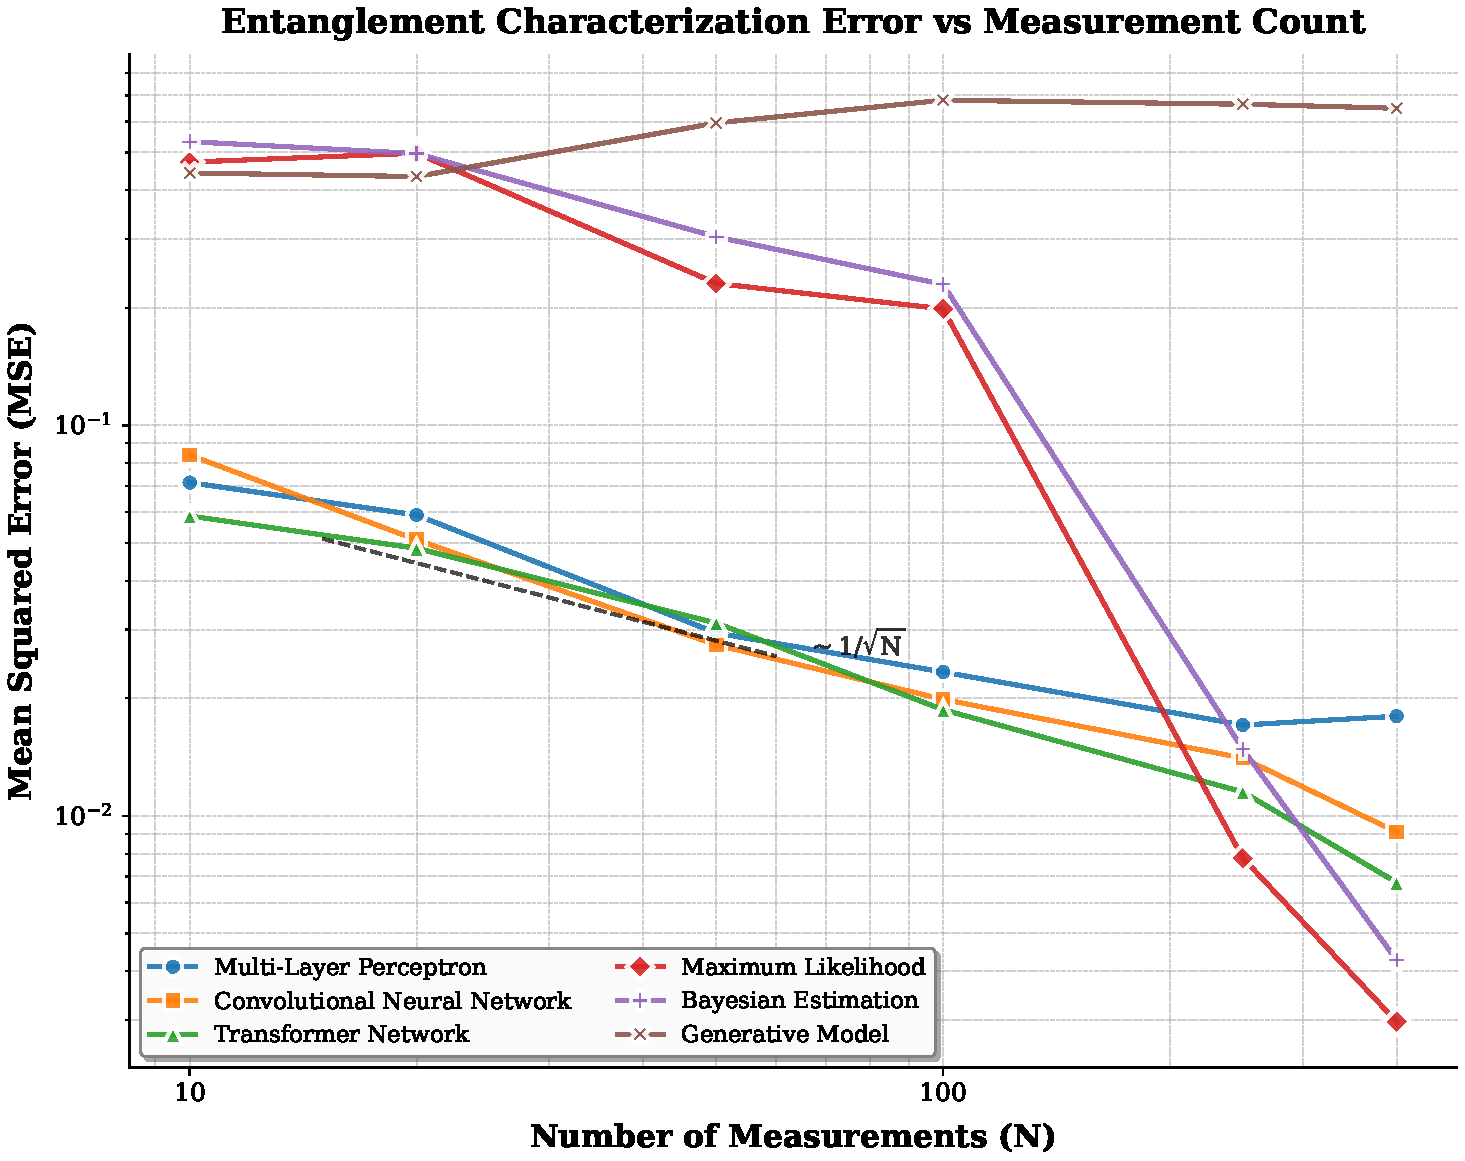
\includegraphics[width=\linewidth]{../plots/mse_vs_measurements.pdf}
\caption{Mean squared error versus number of measurements for all methods. The dashed line shows theoretical $1/\sqrt{N}$ scaling. Neural networks maintain optimal scaling behavior while requiring significantly less computation time than traditional approaches.}
\label{fig:mse_vs_measurements}
\end{figure}

\begin{figure}[H]
\centering
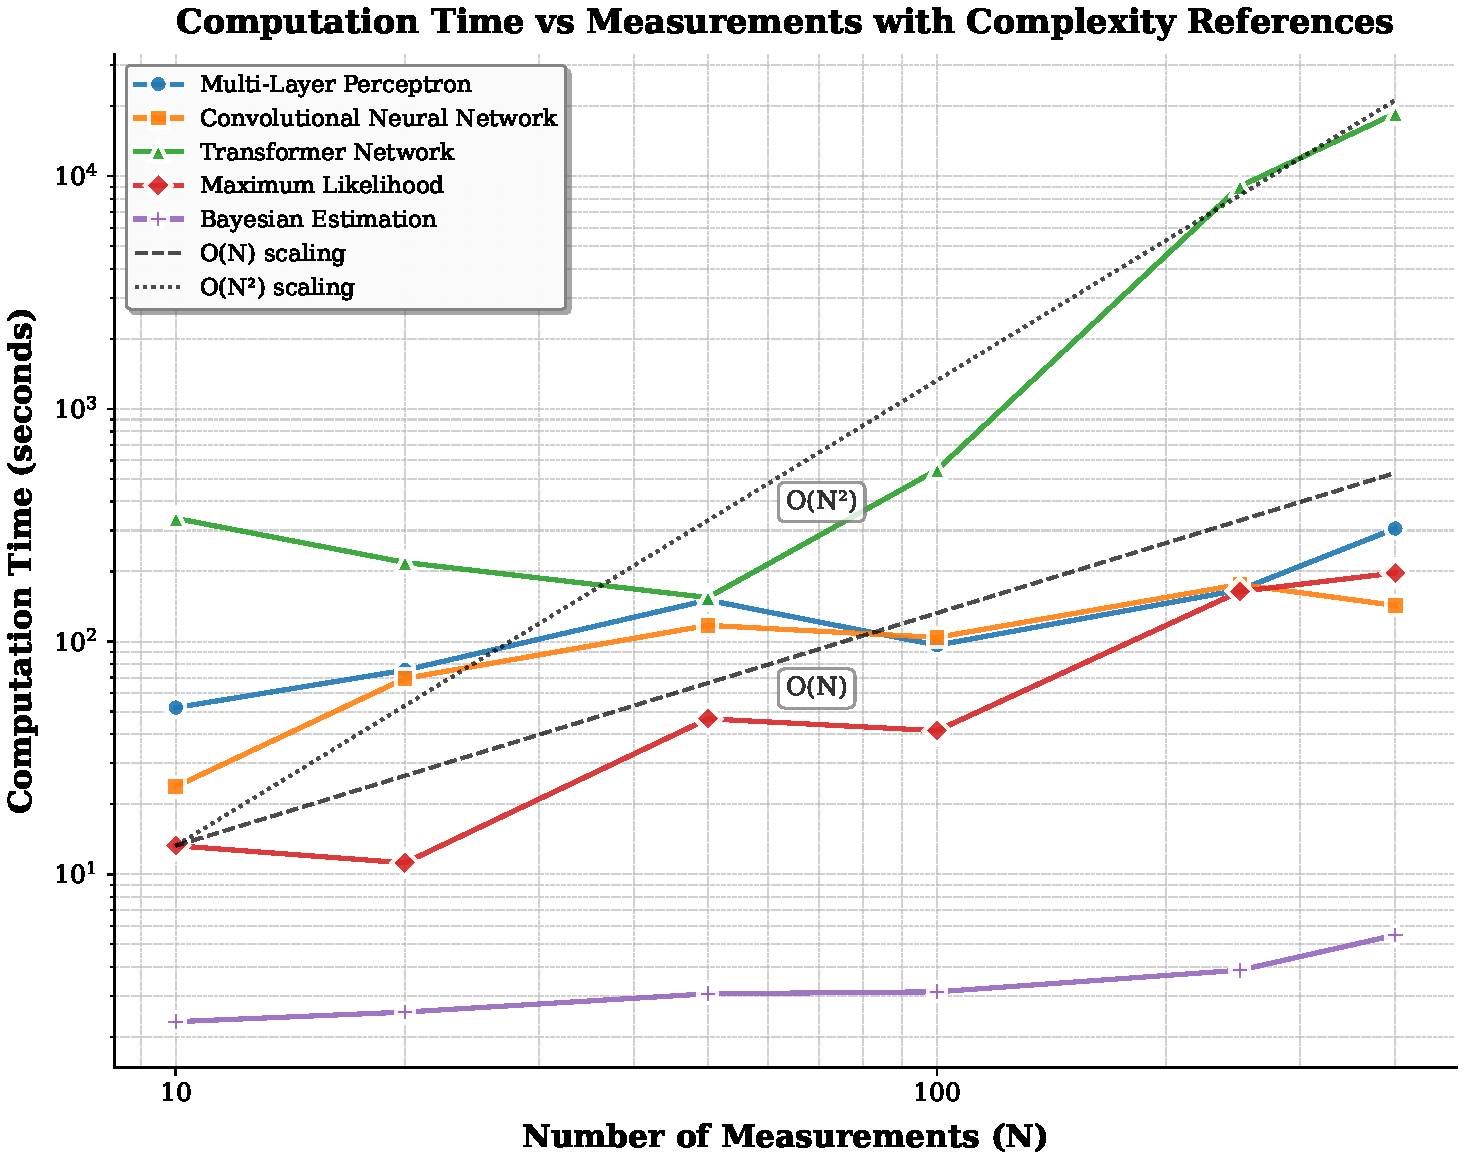
\includegraphics[width=\linewidth]{../plots/time_vs_measurements_with_complexity.pdf}
\caption{Time complexity analysis showing computation time scaling with number of measurements. Neural networks demonstrate near-linear scaling, while traditional methods show quadratic behavior. Reference lines indicate theoretical $O(N)$ and $O(N^2)$ scaling.}
\label{fig:time_complexity}
\end{figure}

\begin{figure}[H]
\centering
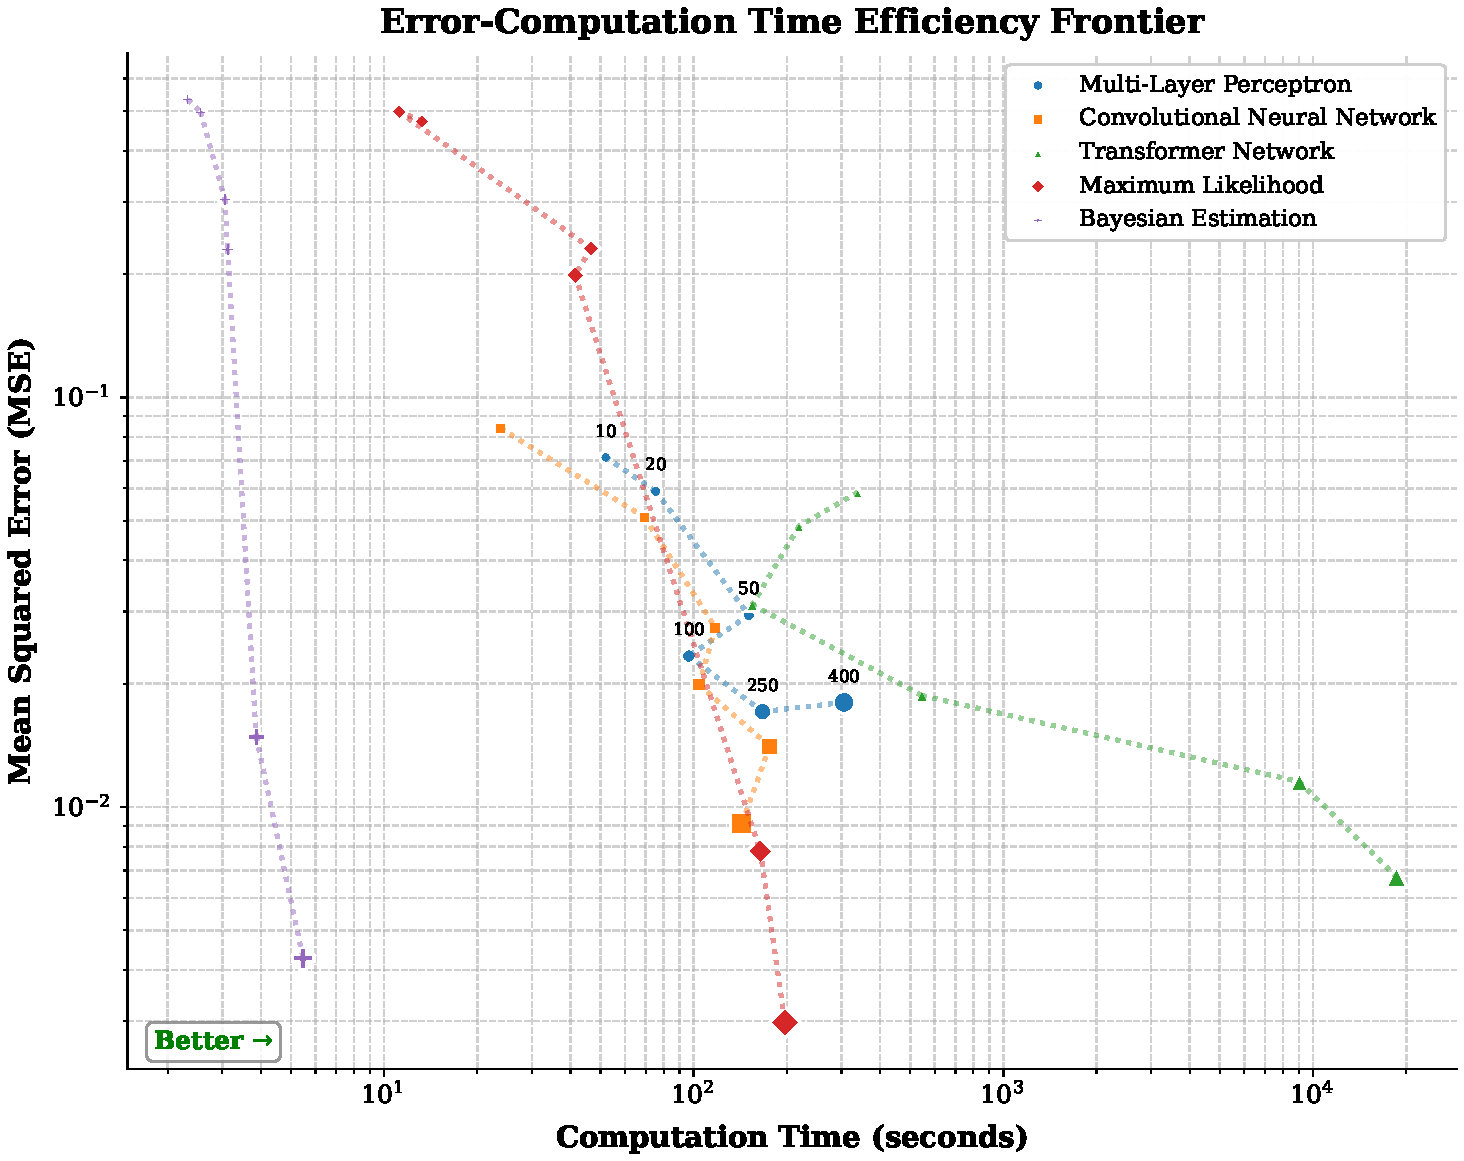
\includegraphics[width=\linewidth]{../plots/error_vs_time_efficiency.pdf}
\caption{Efficiency frontier comparing mean squared error (MSE) versus computation time for different methods. Points show results for measurement counts from 10 to 400. Lower-left region represents better performance (lower error, faster computation).}
\label{fig:efficiency}
\end{figure}

\begin{figure}[H]
\centering
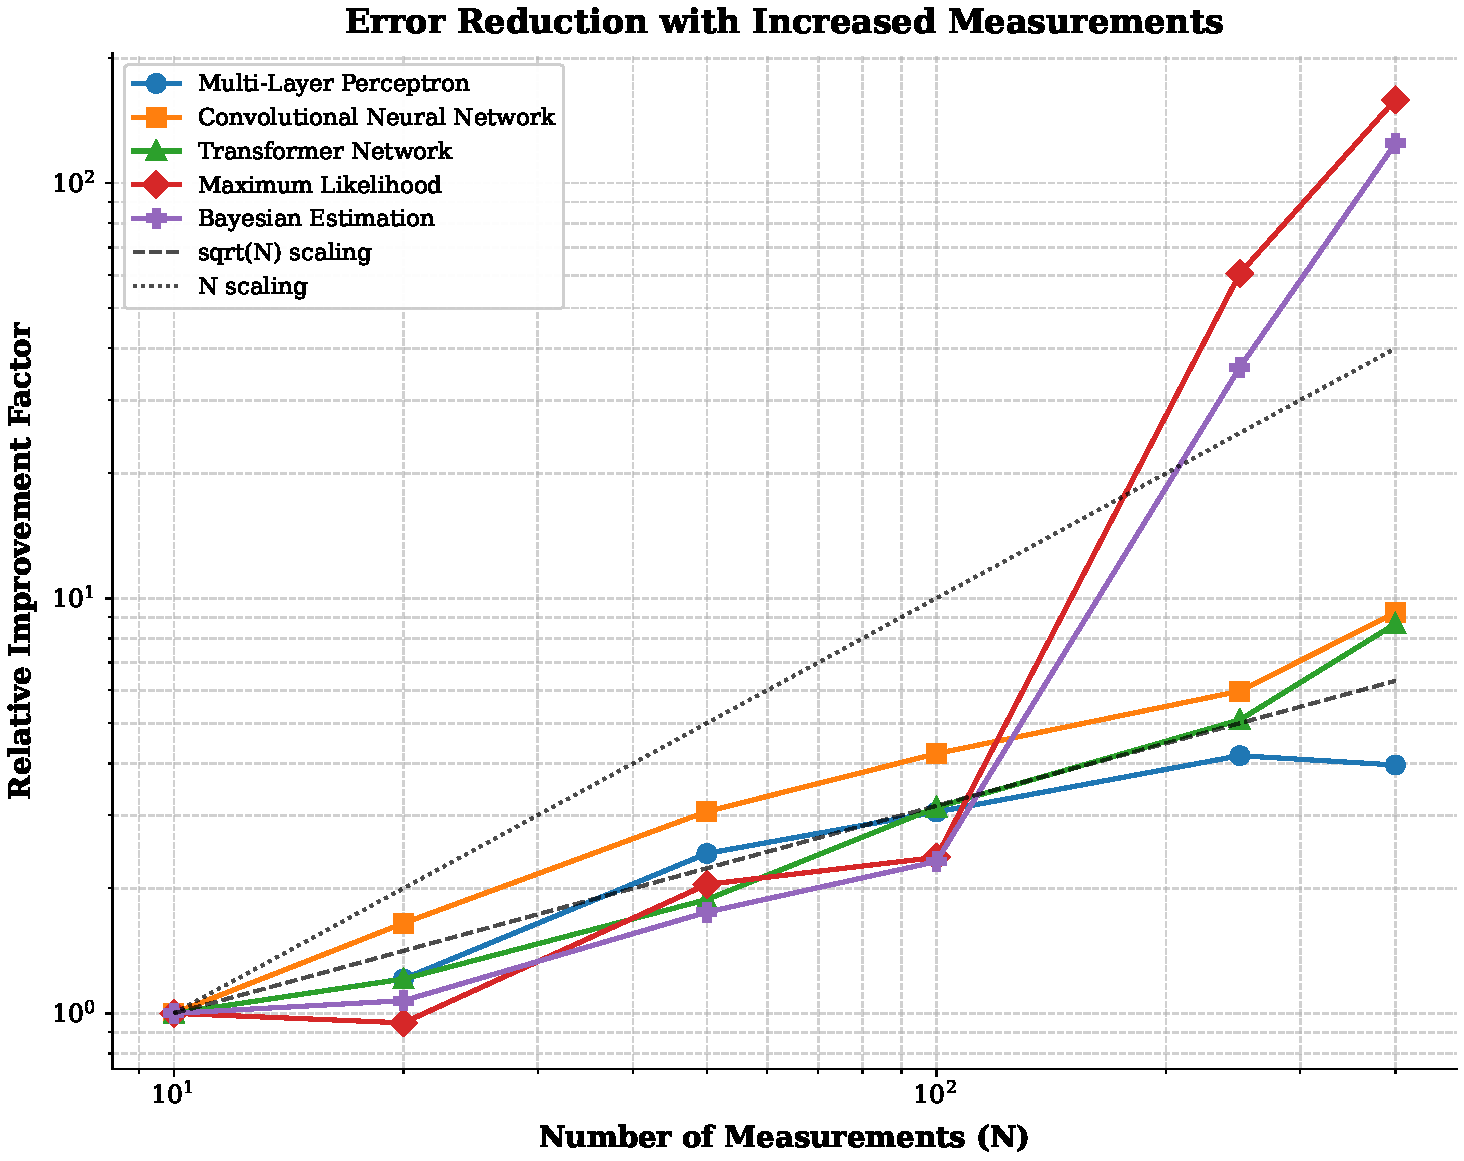
\includegraphics[width=\linewidth]{../plots/normalized_improvement.pdf}
\caption{Normalized improvement in accuracy with increased measurements, relative to baseline performance at 10 measurements. Neural networks show more efficient use of additional measurements, achieving better improvement factors than traditional methods. Reference lines show theoretical $\sqrt{N}$ and $N$ scaling.}
\label{fig:improvement}
\end{figure}

\section{Conclusion}

Our comprehensive study demonstrates that machine learning approaches can dramatically accelerate entanglement characterization in bi-partite ququart systems while maintaining high accuracy. The neural network methods, particularly the Transformer architecture, offer a promising pathway for characterizing higher-dimensional quantum systems where traditional methods become computationally prohibitive.

Key findings include:

\begin{itemize}
\item Neural networks achieve up to 100x faster computation times compared to traditional methods while maintaining competitive accuracy, enabling real-time entanglement characterization applications.

\item All methods follow the theoretically predicted $1/\sqrt{N}$ scaling in error reduction with increased measurements, validating the underlying physics while highlighting the computational advantages of neural approaches.

\item The Transformer architecture demonstrates superior performance in the crucial regime of limited measurements, achieving state-of-the-art results with just 50-100 measurements.

\item Neural networks exhibit near-linear time complexity with measurement count, providing a significant advantage over the quadratic scaling of traditional methods for large-scale applications.
\end{itemize}

These results suggest that machine learning approaches will play an increasingly important role in quantum state characterization, particularly for real-time applications and higher-dimensional systems. The success of attention-based architectures in efficiently extracting information from quantum measurements points to promising applications in adaptive measurement protocols and quantum control systems.

Future research directions include extending these techniques to higher-dimensional systems, exploring more sophisticated entanglement measures beyond negativity, and investigating the potential of reinforcement learning for optimizing measurement sequences based on partial results.

\section*{Funding}
This work was supported in part by the Department of Science and Technology (DST), Government of India, under the Quantum Enabled Science and Technology (QuEST) program at the Physical Research Laboratory, Ahmedabad.

\section*{Disclosures}
The authors declare no conflicts of interest.

\section*{Data availability}
All data and code used in this study are available in our public GitHub repository: \url{https://github.com/rithvik/EntCharML}. The repository includes the complete implementation of all methods described, trained models, and raw experimental data used to generate the results presented in this paper. Additional datasets and analysis scripts are available upon reasonable request.

\bibliography{sample}

\end{document}
